\documentclass[12pt]{article}
\usepackage{geometry}
\geometry{a4paper, total={6in, 9in}} % Ustawienie marginesów
\usepackage{graphicx} % Required for inserting images
\usepackage[utf8]{inputenc} % Kodowanie znaków UTF-8
\usepackage[T1]{fontenc} % Poprawna obsługa polskich znaków
\usepackage[polish]{babel} % Ustawienie języka na polski
\usepackage{parskip} % Dodanie odstępów między paragrafami
\usepackage{titlesec} % Pakiet do kontroli sekcji i formatowania tytułów
\usepackage{fancyhdr} % Nagłówki i stopki
\usepackage{hyperref} % Linki i odniesienia w dokumencie
\usepackage{booktabs} % Lepsze tabele
\usepackage{amsmath} % Obsługa matematyki
\usepackage{setspace} % Zwiększenie odstępów między liniami
\usepackage{indentfirst} % Wcięcie pierwszego akapitu

\title{Zastosowanie konwolucyjnych sieci neuronowych do predykcji wpływu zmian struktury kapitałowej i majątkowej na wartość rynkową przedsiębiorstwa}
\author{Mateusz Łopaciński}
\date{Wrzesień 2024}

\begin{document}

\maketitle

\tableofcontents
\vspace{1cm} % Odstęp między spisem treści a resztą dokumentu

\newpage % Przeniesienie wprowadzenia na nową stronę
\section{Wprowadzenie}

Celem niniejszego raportu jest przedstawienie prac wykonanych w ramach pracowni projektowej, których tematem jest zastosowanie konwolucyjnych sieci neuronowych do predykcji wpływu zmian struktury kapitałowo-majątkowej na wartość rynkową przedsiębiorstwa. W ramach realizacji tego projektu konieczne było zrozumienie podstawowych pojęć związanych z finansami przedsiębiorstw, w szczególności struktury kapitałowej i majątkowej oraz sposobów wyliczania wartości rynkowej spółek giełdowych.

\textbf{Struktura kapitałowo-majątkowa} przedsiębiorstwa obejmuje zasoby i zobowiązania, którymi firma zarządza, a także sposób ich finansowania. Ważnymi elementami tej struktury są m.in.: kapitał własny, zadłużenie długoterminowe oraz aktywa trwałe. Zrozumienie struktury kapitałowej ma istotne znaczenie dla oceny kondycji finansowej przedsiębiorstwa oraz jego wartości na rynku.

\textbf{Wartość rynkowa spółki} najczęściej obliczana jest jako iloczyn ceny rynkowej akcji i liczby wyemitowanych akcji. Ten wskaźnik odzwierciedla wycenę dokonywaną przez inwestorów, która jest uzależniona m.in. od kondycji finansowej, struktury aktywów i pasywów oraz wyników operacyjnych firmy. W projekcie przyjęto tę metodę do obliczania wartości rynkowej spółek giełdowych.

W ramach tego projektu analizowane były rynkowe dane finansowe spółek publikowane w kwartalnych \textbf{bilansach} (balance sheet) notowanych na Giełdzie Papierów Wartościowych w Warszawie z ostatnich 20 lat, obejmujących lata 2004–2024. Dane te zawierały takie zmienne jak aktywa trwałe, kapitał własny, zobowiązania długoterminowe oraz środki pieniężne, które były niezbędne do stworzenia modelu predykcyjnego.

\newpage % Przeniesienie wprowadzenia na nową stronę
\section{Pobieranie danych}

W trakcie realizacji projektu konieczne było pozyskanie danych finansowych spółek giełdowych. Początkowo rozważana była możliwość wykorzystania danych dostępnych w statystykach publikowanych na stronie GPW\footnote{\url{https://www.gpw.pl/statystyki-gpw}, dostęp: 8 września 2024}. Niestety, dane te nie zawierały wystarczających informacji dotyczących struktury kapitałowo-majątkowej przedsiębiorstw, co było kluczowe dla realizacji projektu.

\subsection{Próba wykorzystania eksportera danych}

Podjęta została także próba użycia narzędzia eksportera danych, który został załączony w plikach pomocniczych, jednakże próba jego wykorzystania kończyła się błędami, co uniemożliwiło dalsze jego użycie w projekcie.

\subsection{Wykorzystanie API FinancialModelingPrep}

Ze względu na powyższe trudności, podjęta została decyzja o wykorzystaniu API dostępnego na stronie FinancialModelingPrep\footnote{\url{https://site.financialmodelingprep.com/}, dostęp: 8 września 2024}. API to oferuje szeroki dostęp do danych finansowych spółek giełdowych z całego świata, w tym również z GPW. Udało się pozyskać dane dotyczące 396 spółek notowanych na GPW.

\subsection{Proces pobierania danych}

W pierwszej kolejności pobrana została lista wszystkich spółek dostępnych w API\footnote{\url{https://financialmodelingprep.com/api/v3/stock/list}, dostęp: 8 września 2024}. Następnie, po odfiltrowaniu spółek GPW na podstawie nazwy giełdy, uzyskany został dostęp do danych finansowych, w tym bilansów\footnote{\url{https://financialmodelingprep.com/api/v3/balance-sheet-statement}, dostęp: 8 września 2024}. Dane te obejmowały okres 20 lat w ujęciu kwartalnym, co pozwoliło na zbudowanie szczegółowej bazy do dalszych analiz.

\subsection{Obliczanie wartości rynkowej spółki}

Wartość rynkowa spółki została obliczona jako iloczyn ceny akcji (\emph{stock price}) oraz liczby wyemitowanych akcji (\emph{shares outstanding}). Do pobrania historycznych danych na temat cen akcji wykorzystany został odpowiedni endpoint API\footnote{\url{https://financialmodelingprep.com/api/v3/historical-price-full}, dostęp: 8 września 2024}. Dzięki temu możliwe było uzyskanie pełnego obrazu zmian wartości rynkowej każdej z analizowanych spółek.

\newpage % Przeniesienie na nową stronę
\section{Preprocessing danych}

W celu odpowiedniego przygotowania danych do trenowania modelu, konieczne było przeprowadzenie kilku kroków wstępnych, mających na celu eliminację niepotrzebnych lub zaburzających dane elementów.

\subsection{Eliminacja wierszy o innej walucie niż PLN}

Pierwszym krokiem było wyeliminowanie wierszy, które zawierały dane finansowe w walutach innych niż PLN. Dane te zaburzyłyby działanie modelu, ponieważ wartości wyrażone w różnych walutach nie są porównywalne bez wcześniejszej konwersji. Ponieważ jednak liczba takich wierszy była niewielka, zdecydowano się na ich usunięcie, co było prostsze i bardziej efektywne niż konwersja walut z ostatnich 20 lat.

\subsection{Eliminacja kolumn nienumerycznych}

Następnie odrzucono kolumny zawierające dane nienumeryczne, które nie były potrzebne do dalszej analizy. Oto lista kolumn wraz z tłumaczeniem:
\begin{itemize}
    \item \textbf{reportedCurrency} – Waluta raportu
    \item \textbf{cik} – Numer identyfikacyjny spółki
    \item \textbf{fillingDate} – Data wypełnienia formularza
    \item \textbf{acceptedDate} – Data akceptacji formularza
    \item \textbf{calendarYear} – Rok kalendarzowy
    \item \textbf{finalLink} – Link do ostatecznego raportu
    \item \textbf{link} – Link do raportu
    \item \textbf{period} – Okres raportu
\end{itemize}

\subsection{Odrzucenie spółek z krótkim okresem notowań}

Odrzucono spółki, które były notowane na giełdzie przez okres krótszy niż 2 lata. Spółki te miały zbyt krótki okres istnienia, aby można było wyciągać z nich miarodajne wnioski dotyczące zmian w strukturze kapitałowo-majątkowej.

Po tej redukcji, pozostało 375 spółek.

\subsection{Eliminacja kolumn zawierających sumy innych kolumn}

W kolejnym kroku odrzucono kolumny zawierające sumy innych zmiennych, aby uniknąć nadmiarowych danych:
\begin{itemize}
    \item \textbf{cashAndShortTermInvestments} – suma \emph{Gotówka i Ekwiwalenty Gotówki} oraz \emph{Inwestycje Krótkoterminowe}
    \item \textbf{goodwillAndIntangibleAssets} – suma \emph{Wartość Firmy} oraz \emph{Wartości Niematerialne}
    \item \textbf{totalLiabilitiesAndStockholdersEquity} – suma \emph{Kapitał Własny Akcjonariuszy} oraz \emph{Całkowity Kapitał Własny}
    \item \textbf{totalLiabilitiesAndTotalEquity} – suma \emph{Całkowity Kapitał Własny} oraz \emph{Suma Zobowiązań}
\end{itemize}

\subsection{Odrzucenie kolumn z symbolem i datą raportu}

W dalszej części procesu, usunięto kolumny zawierające symbol spółki oraz daty raportu, aby pozostały tylko wartości numeryczne. Następnie stworzono macierz korelacji Pearsona (zob. Rysunek \ref{fig:pearson_corr}), co pozwoliło zidentyfikować silnie skorelowane cechy.

\begin{figure}[h]
    \centering
    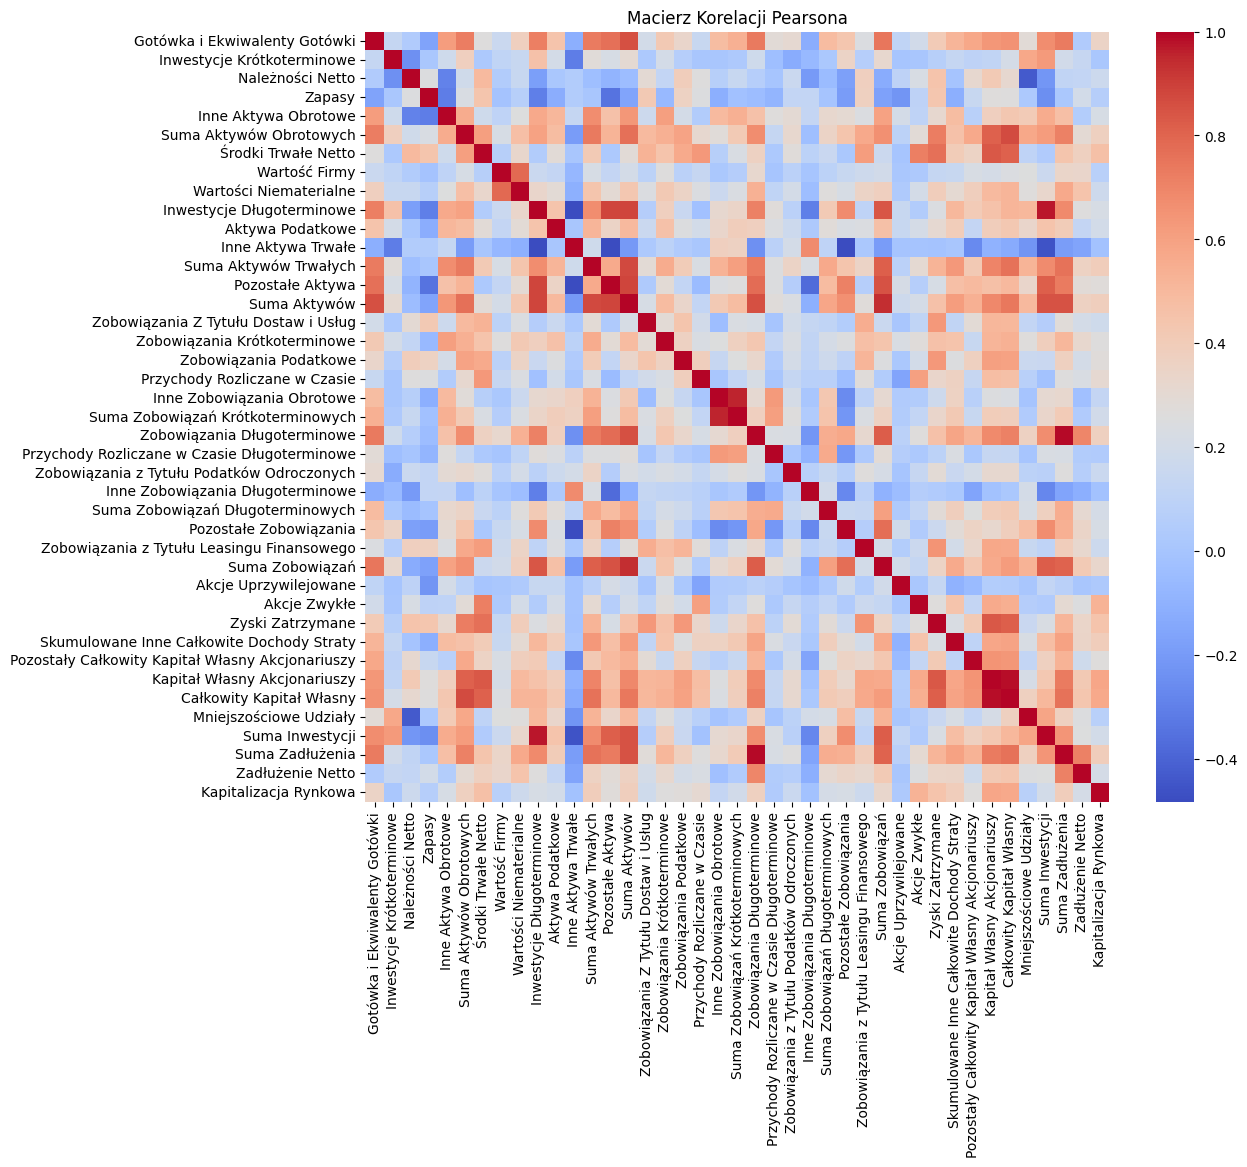
\includegraphics[width=0.8\textwidth]{docs/img/pearson-correlation.png}
    \caption{Macierz korelacji Pearsona}
    \label{fig:pearson_corr}
\end{figure}

\subsection{Eliminacja skorelowanych cech}

Zidentyfikowano pary cech o wysokiej korelacji, z których jedna została odrzucona, aby zapobiec nadmiernej redundancji danych. Odrzucono następujące kolumny:
\begin{itemize}
    \item \textbf{otherCurrentLiabilities} (\emph{Inne Zobowiązania Obrotowe}) – zdecydowano się na pozostawienie \emph{totalCurrentLiabilities}, ponieważ obejmuje szerszą kategorię zobowiązań krótkoterminowych.
    \item \textbf{longTermDebt} (\emph{Zobowiązania Długoterminowe}) – zdecydowano się na pozostawienie \emph{totalDebt}, który obejmuje całkowite zadłużenie (zarówno długoterminowe, jak i krótkoterminowe).
    \item \textbf{totalStockholdersEquity} (\emph{Kapitał Własny Akcjonariuszy}) – zdecydowano się na pozostawienie \emph{totalEquity}, który opisuje bardziej ogólnie całkowity kapitał własny, obejmujący nie tylko akcjonariuszy.
    \item \textbf{longTermInvestments} (\emph{Inwestycje Długoterminowe}) – zdecydowano się na pozostawienie \emph{totalInvestments}, który obejmuje wszystkie inwestycje, zarówno krótkoterminowe, jak i długoterminowe.
\end{itemize}

\subsection{Eliminacja mało istotnych cech}

Na kolejnym etapie stworzono wykres istotności cech (zob. Rysunek \ref{fig:feature_importance}), co pozwoliło na identyfikację zmiennych o niskiej wartości istotności. Dla cech, które miały wartość poniżej ustalonego progu \emph{importance\_threshold = 0.005}, dokonano ich eliminacji.

\begin{figure}[h]
    \centering
    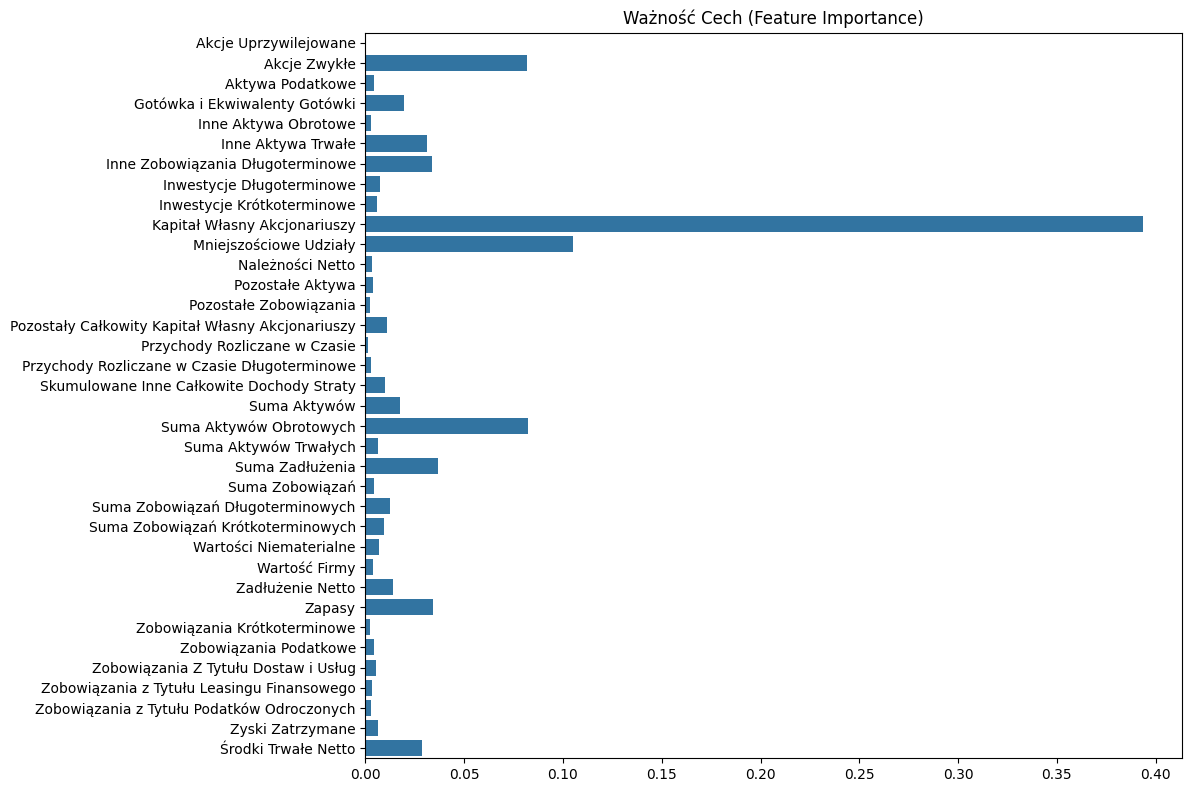
\includegraphics[width=0.8\textwidth]{docs/img/feature-importances.png}
    \caption{Wykres istotności cech}
    \label{fig:feature_importance}
\end{figure}

Odrzucono następujące cechy:
\begin{itemize}
    \item Akcje Uprzywilejowane (\emph{preferredStock})
    \item Aktywa Podatkowe (\emph{taxAssets})
    \item Inne Aktywa Obrotowe (\emph{otherCurrentAssets})
    \item Inwestycje Krótkoterminowe (\emph{shortTermInvestments})
    \item Należności Netto (\emph{netReceivables})
    \item Pozostałe Aktywa (\emph{otherAssets})
    \item Pozostałe Zobowiązania (\emph{otherLiabilities})
    \item Przychody Rozliczane w Czasie (\emph{deferredRevenue})
    \item Przychody Rozliczane w Czasie Długoterminowe (\emph{deferredRevenueNonCurrent})
    \item Zobowiązania Krótkoterminowe (\emph{shortTermDebt})
    \item Zobowiązania Podatkowe (\emph{taxPayables})
    \item Zobowiązania z Tytułu Leasingu Finansowego (\emph{capitalLeaseObligations})
    \item Zobowiązania z Tytułu Podatków Odroczonych (\emph{deferredTaxLiabilitiesNonCurrent})
    \item Zyski Zatrzymane (\emph{retainedEarnings})
\end{itemize}

\subsection{Skalowanie danych i usunięcie outlierów}

Ostatnim krokiem w preprocessingu było skalowanie danych z użyciem \emph{StandardScaler}. Dane zapisano w dwóch wariantach:
\begin{enumerate}
    \item Dane przeskalowane bez wcześniejszych modyfikacji.
    \item Dane, w których przed skalowaniem odrzucono outliery przy użyciu algorytmu LOF (\emph{Local Outlier Factor}), a następnie przeskalowano z wykorzystaniem \emph{StandardScaler}.
\end{enumerate}

Przekształcone dane zapisano do plików CSV i były one gotowe do użycia podczas trenowania modelu CNN.

\end{document}
